\section{システム開発と設計}

\subsection{手法}

\paragraph {従来のmy\_help,wiki,latex}
\begin{figure}[htbp]\begin{center}
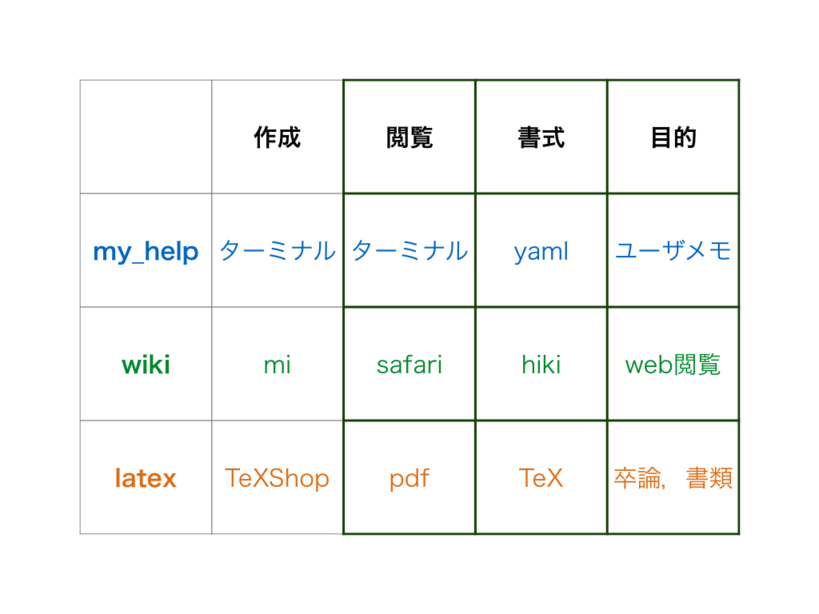
\includegraphics[width=6cm,bb=100 100 600 700]{my_help2hiki_saki.003.png}
\caption{ my\_help,wiki,latexの比較}
\label{default}\end{center}\end{figure}
\begin{description}
\item 上図はmy\_help,wiki,latexの作成,閲覧,書式,目的を比較した図である.
\end{description}
\begin{itemize}
\item my\_help
\end{itemize}
\begin{description}
\item my\_helpは,メモを作るためのgem.
ユーザがターミナルを利用して作成し,閲覧する.
メモの書式はyaml形式で,拡張子は.ymlを使用している.
\end{description}

\begin{itemize}
\item wiki
\end{itemize}
\begin{description}
\item miというmacのテキストエディタを用いて作成する.
作成したファイルはMac OSのブラウザのsafariで開くことができる.
hiki形式で記述し,webを通して誰でも見られるようにできる.
\end{description}

\begin{itemize}
\item latex
\end{itemize}
\begin{description}
\item TeXの書式で,TeX編集用エディタのTeXShopによって作成する.
pdfは一般的に使われている電子ファイルで,印刷して卒業論文の
ハードコピーとしても使われる.
\end{description}

このようにmy\_help,wiki,latexは書式や作成,閲覧方法が全て違う.
目的も異なるので,同じ内容のファイルをそれぞれの書式で書かなければならないことがある.

\begin{figure}[htbp]\begin{center}
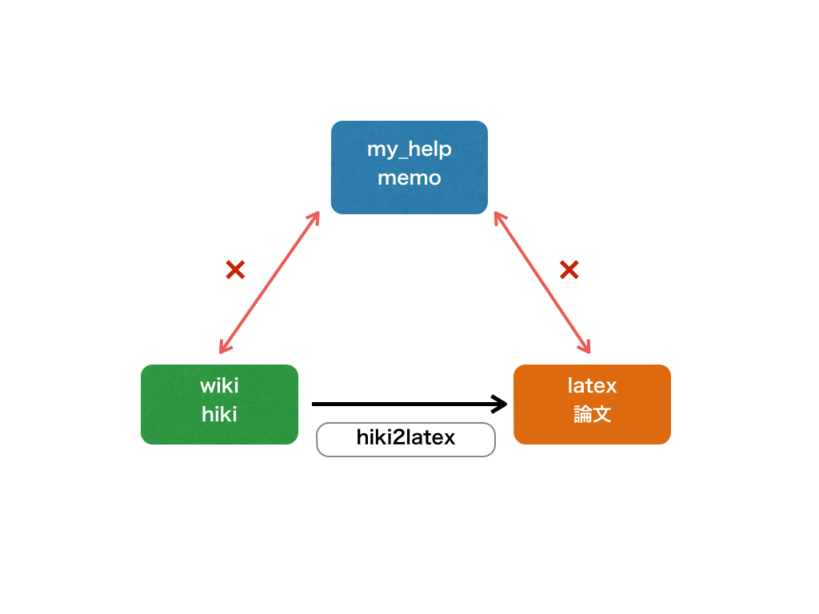
\includegraphics[width=6cm,bb=100 100 600 700]{my_help2hiki_saki.004.png}
\caption{ hiki2latex}
\label{default}\end{center}\end{figure}
hiki2latexの開発により図4のようにwikiとlatexの変換はできるようになったが,
my\_helpとwiki,my\_helpとlatexは関連させることができなかった.
本研究により,my\_help,wiki,latexを関連させるため,
my\_helpからwikiへ自動変換を行うシステムmy\_help2hikiの開発を目指す.

\begin{figure}[htbp]\begin{center}
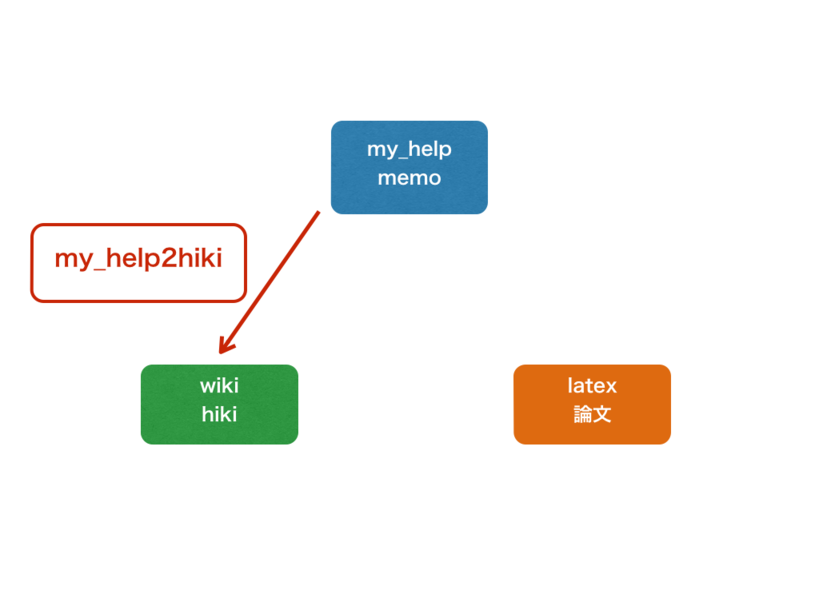
\includegraphics[width=6cm,bb=0 0 442 500]{my_help2hiki_saki.005.png}
\caption{my\_help2hiki}
\label{default}\end{center}\end{figure}